\documentclass[aspectratio=169]{beamer}

\usetheme{Madrid}
\usecolortheme{default}

\usepackage{tikz}
\usetikzlibrary{shapes.geometric,arrows.meta,positioning,fit,backgrounds,calc}
\usepackage{listings}
\usepackage{graphicx}
\usepackage{booktabs}
\usepackage{xcolor}
\usepackage{amsmath}
\usepackage{microtype}

% ── Colours ──────────────────────────────────────────────────────────────────
\definecolor{nwblue}{RGB}{30,100,180}
\definecolor{swred}{RGB}{180,30,30}
\definecolor{passgrn}{RGB}{30,140,60}
\definecolor{hashbg}{RGB}{220,240,255}
\definecolor{loopbg}{RGB}{255,235,210}
\definecolor{hdrblue}{RGB}{200,225,255}

% ── Listings style ────────────────────────────────────────────────────────────
\lstdefinestyle{bashstyle}{
  language=bash,
  basicstyle=\ttfamily\tiny,
  keywordstyle=\color{blue!70!black},
  commentstyle=\itshape\color{gray},
  breaklines=true,
  frame=single,
  rulecolor=\color{gray!30},
  xleftmargin=2pt, xrightmargin=2pt,
  morekeywords={clang,opt,llc,aarch64-gcc}
}
\lstdefinestyle{logstyle}{
  basicstyle=\ttfamily\tiny,
  breaklines=true,
  frame=single,
  rulecolor=\color{gray!30},
  xleftmargin=2pt, xrightmargin=2pt
}

% ── Meta ─────────────────────────────────────────────────────────────────────
\title[C-FLAT on ARM TrustZone]
      {C-FLAT: Control Flow Attestation for Embedded Systems}
\subtitle{Implementation and Evaluation on ARM TrustZone / Raspberry Pi~3}
\author{Rajesh}
\institute{}
\date{\today}

% ─────────────────────────────────────────────────────────────────────────────
\begin{document}

% ══════════════════════════════════════════════════════════════════════════════
% SLIDE 1 — TITLE
% ══════════════════════════════════════════════════════════════════════════════
\begin{frame}
  \titlepage
\end{frame}

% ══════════════════════════════════════════════════════════════════════════════
% SLIDE 2 — PROBLEM STATEMENT
% ══════════════════════════════════════════════════════════════════════════════
\begin{frame}{Motivation: The Limits of Static Security Guarantees}
\begin{columns}[T]

\begin{column}{0.57\textwidth}
  \textbf{Code signing / binary attestation is not enough:}
  \begin{itemize}
    \item Verifies \emph{what} code is loaded — not \emph{how} it executes
    \item \textbf{Return-Oriented Programming (ROP) / JOP:} reuse existing code
          gadgets without injecting new code
    \item Binary is unchanged $\Rightarrow$ static attestation \emph{passes}
    \item Execution follows an \emph{unauthorised} path through the CFG
  \end{itemize}

  \bigskip
  \textbf{Standard CFI also falls short:}
  \begin{itemize}
    \item Enforces valid call/return \emph{targets}, not the complete path
    \item Does \emph{not} detect data-oriented attacks \\
          (e.g.\ loop counter corruption to dispense wrong drug dose)
  \end{itemize}

  \bigskip
  \textbf{Research Question:}
  \begin{quote}
    \itshape Can we cryptographically prove that a program executed its
    intended control-flow path, including correct loop counts, at runtime?
  \end{quote}
\end{column}

\begin{column}{0.37\textwidth}
  \centering
  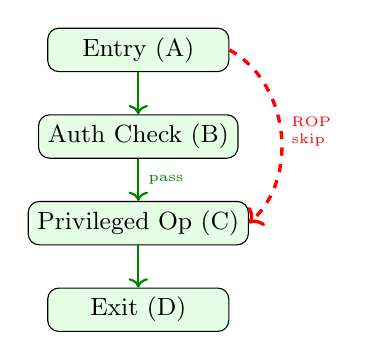
\begin{tikzpicture}[font=\small, node distance=1.1cm,
      bb/.style={draw,rounded corners,minimum width=2.3cm,
                 minimum height=0.55cm,align=center}]
    \node[bb,fill=green!10]  (A) {Entry (A)};
    \node[bb,fill=green!10, below of=A] (B) {Auth Check (B)};
    \node[bb,fill=green!10, below of=B] (C) {Privileged Op (C)};
    \node[bb,fill=green!10, below of=C] (D) {Exit (D)};

    \draw[->,thick,green!50!black] (A)--(B);
    \draw[->,thick,green!50!black] (B)--node[right,font=\tiny]{pass}(C);
    \draw[->,thick,green!50!black] (C)--(D);

    % ROP arc
    \draw[->,very thick,red,dashed]
      (A.east) to[bend left=55]
      node[right,font=\tiny,red,align=left]{ROP\\skip}
      (C.east);
  \end{tikzpicture}

  \vspace{0.6em}
  {\footnotesize\itshape ROP skips the auth check.
  The binary is unmodified; static attestation passes.
  C-FLAT detects this via a hash mismatch.}
\end{column}

\end{columns}
\end{frame}

% ══════════════════════════════════════════════════════════════════════════════
% SLIDE 3 — BACKGROUND: C-FLAT & TRUSTZONE
% ══════════════════════════════════════════════════════════════════════════════
\begin{frame}{Background: C-FLAT and ARM TrustZone}
\begin{columns}[T]

\begin{column}{0.52\textwidth}
  \textbf{C-FLAT (CCS 2017) — extended in BLAST (CCS 2023):}
  \begin{itemize}
    \item Instrument the binary to record every CFG edge traversal
    \item Compute a cryptographic \emph{authenticator} of the execution path
    \item Isolate the measurement engine inside a hardware trust anchor
    \item Verifier checks authenticator against a pre-computed ``golden'' value
  \end{itemize}

  \bigskip
  \textbf{Our Implementation:}
  \begin{itemize}
    \item \textbf{Platform:} Raspberry Pi~3 (BCM2837, AArch64) with OP-TEE~v4.x
    \item \textbf{Instrumentation:} LLVM IR-level pass \\
          (original paper used binary rewriting on ARMv7)
    \item \textbf{Measurement Engine:} OP-TEE Trusted Application using
          hardware SHA-256 via TEE Crypto API
    \item \textbf{Validation target:} Table~2 of BLAST (CCS 2023)
  \end{itemize}
\end{column}

\begin{column}{0.44\textwidth}
  \centering
  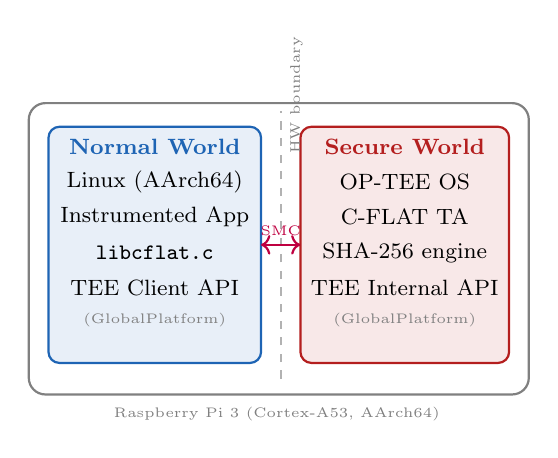
\begin{tikzpicture}[font=\footnotesize]
    % Outer RPi3 board
    \draw[gray,thick,rounded corners=6pt]
      (-0.25,-0.4) rectangle (6.1,3.3);
    \node[gray,font=\tiny] at (2.9,-0.65)
      {Raspberry Pi~3 (Cortex-A53, AArch64)};

    % Normal World box
    \draw[fill=nwblue!10,draw=nwblue,thick,rounded corners=4pt]
      (0,0) rectangle (2.7,3.0);
    \node[font=\footnotesize\bfseries,nwblue] at (1.35,2.75) {Normal World};
    \node at (1.35,2.3)  {Linux (AArch64)};
    \node at (1.35,1.85) {Instrumented App};
    \node at (1.35,1.4)  {\texttt{libcflat.c}};
    \node at (1.35,0.95) {TEE Client API};
    \node[font=\tiny,gray] at (1.35,0.55) {(GlobalPlatform)};

    % Secure World box
    \draw[fill=swred!10,draw=swred,thick,rounded corners=4pt]
      (3.2,0) rectangle (5.85,3.0);
    \node[font=\footnotesize\bfseries,swred] at (4.525,2.75) {Secure World};
    \node at (4.525,2.3)  {OP-TEE OS};
    \node at (4.525,1.85) {C-FLAT TA};
    \node at (4.525,1.4)  {SHA-256 engine};
    \node at (4.525,0.95) {TEE Internal API};
    \node[font=\tiny,gray] at (4.525,0.55) {(GlobalPlatform)};

    % HW boundary + SMC arrow
    \draw[dashed,gray!60,thick] (2.95,-0.2)--(2.95,3.2);
    \node[gray,font=\tiny,rotate=90] at (3.15,3.4) {HW boundary};
    \draw[<->,purple,thick] (2.7,1.5)--(3.2,1.5);
    \node[purple,font=\tiny,above] at (2.95,1.5) {SMC};
  \end{tikzpicture}
\end{column}

\end{columns}
\end{frame}

% ══════════════════════════════════════════════════════════════════════════════
% SLIDE 4 — SYSTEM ARCHITECTURE
% ══════════════════════════════════════════════════════════════════════════════
\begin{frame}{System Architecture}
\centering
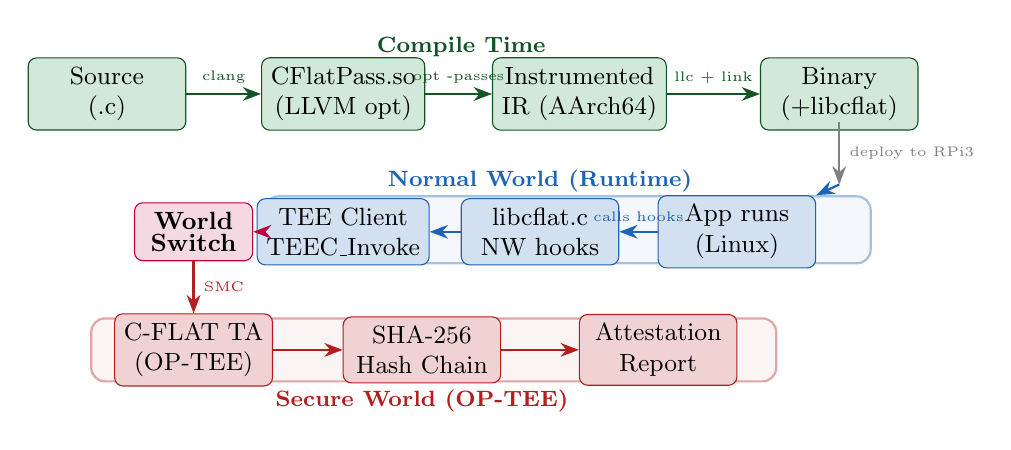
\begin{tikzpicture}[
    cbox/.style={draw,rounded corners=3pt,minimum width=2.0cm,
                 minimum height=0.65cm,align=center,font=\small},
    arr/.style={->,thick,>=Stealth},
    font=\small
  ]

  %% ── Compile-time row ──────────────────────────────────────────────────────
  \node[cbox,fill=passgrn!20,draw=passgrn!60!black] (src)
      at (0,2.5)   {Source\\(.c)};
  \node[cbox,fill=passgrn!20,draw=passgrn!60!black] (pass)
      at (3.0,2.5) {CFlatPass.so\\(LLVM opt)};
  \node[cbox,fill=passgrn!20,draw=passgrn!60!black] (ir)
      at (6.0,2.5) {Instrumented\\IR (AArch64)};
  \node[cbox,fill=passgrn!20,draw=passgrn!60!black] (bin)
      at (9.3,2.5) {Binary\\(+libcflat)};

  \draw[arr,passgrn!60!black] (src)  -- node[above,font=\tiny]{clang}     (pass);
  \draw[arr,passgrn!60!black] (pass) -- node[above,font=\tiny]{opt -passes} (ir);
  \draw[arr,passgrn!60!black] (ir)   -- node[above,font=\tiny]{llc + link} (bin);
  \node[passgrn!60!black,font=\footnotesize\bfseries] at (4.5,3.1) {Compile Time};

  %% ── Deploy arrow ──────────────────────────────────────────────────────────
  \draw[arr,gray,thick] (9.3,2.15) -- (9.3,1.35)
      node[midway,right,font=\tiny]{deploy to RPi3};

  %% ── Normal World row ──────────────────────────────────────────────────────
  \node[cbox,fill=nwblue!20,draw=nwblue] (app)
      at (8.0,0.75) {App runs\\(Linux)};
  \node[cbox,fill=nwblue!20,draw=nwblue] (lib)
      at (5.5,0.75) {libcflat.c\\NW hooks};
  \node[cbox,fill=nwblue!20,draw=nwblue] (teec)
      at (3.0,0.75) {TEE Client\\TEEC\_Invoke};

  \draw[arr,nwblue] (9.3,1.35) -- (app);
  \draw[arr,nwblue] (app)  -- node[above,font=\tiny]{calls hooks} (lib);
  \draw[arr,nwblue] (lib)  -- (teec);
  \node[nwblue,font=\footnotesize\bfseries] at (5.5,1.4) {Normal World (Runtime)};

  %% ── World switch ──────────────────────────────────────────────────────────
  \node[cbox,fill=purple!15,draw=purple,minimum width=1.5cm] (ws)
      at (1.1,0.75) {\textbf{World}\\[-3pt]\textbf{Switch}};
  \draw[arr,purple] (teec) -- (ws);

  %% ── Secure World row ──────────────────────────────────────────────────────
  \node[cbox,fill=swred!20,draw=swred] (ta)
      at (1.1,-0.75) {C-FLAT TA\\(OP-TEE)};
  \node[cbox,fill=swred!20,draw=swred] (hsh)
      at (4.0,-0.75) {SHA-256\\Hash Chain};
  \node[cbox,fill=swred!20,draw=swred] (rpt)
      at (7.0,-0.75) {Attestation\\Report};

  \draw[arr,swred] (ws)  -- node[right,font=\tiny]{SMC} (ta);
  \draw[arr,swred] (ta)  -- (hsh);
  \draw[arr,swred] (hsh) -- (rpt);
  \node[swred,font=\footnotesize\bfseries] at (4.0,-1.4) {Secure World (OP-TEE)};

  %% ── Background fills ──────────────────────────────────────────────────────
  \begin{pgfonlayer}{background}
    \fill[nwblue!5,rounded corners=5pt]  (2.0,0.35) rectangle (9.7,1.2);
    \draw[nwblue!40,thick,rounded corners=5pt] (2.0,0.35) rectangle (9.7,1.2);
    \fill[swred!5,rounded corners=5pt]  (-0.2,-1.15) rectangle (8.5,-0.35);
    \draw[swred!40,thick,rounded corners=5pt] (-0.2,-1.15) rectangle (8.5,-0.35);
  \end{pgfonlayer}

\end{tikzpicture}
\end{frame}

% ══════════════════════════════════════════════════════════════════════════════
% SLIDE 5 — LLVM INSTRUMENTATION PASS
% ══════════════════════════════════════════════════════════════════════════════
\begin{frame}[fragile]{LLVM Instrumentation Pass (\texttt{CFlatPass.cpp})}
\begin{columns}[T]

\begin{column}{0.48\textwidth}
  \textbf{Four CFG edge types instrumented at IR level:}

  \medskip
  \begin{tabular}{@{}lll@{}}
    \toprule
    \textbf{Edge Type}    & \textbf{Hook}           & \textbf{Args}         \\
    \midrule
    Conditional branch    & \texttt{record\_node}   & BB id                 \\
    Unconditional branch  & \texttt{record\_node}   & BB id                 \\
    Direct function call  & \texttt{call\_enter}    & call id, caller BB    \\
    Function return       & \texttt{call\_return}   & BB id                 \\
    \bottomrule
  \end{tabular}

  \medskip
  \begin{itemize}
    \item BB ID = first-instruction pointer in the IR (stable, unique)
    \item Skips: intrinsics, external calls, indirect calls, runtime stubs
    \item \textbf{Loops} = back-edges $\Rightarrow$ covered by \texttt{record\_node};
          no separate loop event needed
  \end{itemize}

  \medskip
  \textbf{Example pass diagnostic output:}
  \begin{lstlisting}[style=logstyle]
[CFLAT] bolus | branches=14 calls=4 returns=1
[CFLAT] main  | branches=6  calls=3 returns=1
  \end{lstlisting}
\end{column}

\begin{column}{0.49\textwidth}
  \textbf{Six-step build pipeline (per benchmark):}

  \begin{lstlisting}[style=bashstyle]
# 1. Source -> LLVM IR (AArch64 cross-compile)
clang -S -emit-llvm -O0 \
  --target=aarch64-linux-gnu \
  -Xclang -disable-O0-optnone \
  app.c -o app.ll

# 2. Apply C-FLAT instrumentation pass
opt -load-pass-plugin=CFlatPass.so \
    -passes=cflat-pass \
    app.ll -S -o app_instrumented.ll

# 3. Instrumented IR -> AArch64 object
llc -march=aarch64 -filetype=obj \
    app_instrumented.ll -o app.o

# 4. Compile wrapper (main + cflat_finalize)
clang ... wrapper.c -o wrapper.ll
opt  -passes=cflat-pass wrapper.ll ...
llc  -filetype=obj wrapper_inst.ll ...

# 5. Link: obj + wrapper + libcflat + libteec
aarch64-gcc app.o wrapper.o libcflat.o \
    -lteec -o cflat_app
  \end{lstlisting}
\end{column}

\end{columns}
\end{frame}

% ══════════════════════════════════════════════════════════════════════════════
% SLIDE 6 — TRUSTED APPLICATION
% ══════════════════════════════════════════════════════════════════════════════
\begin{frame}{Trusted Application: Measurement Engine (\texttt{cflat\_ta.c})}
\begin{columns}[T]

\begin{column}{0.50\textwidth}
  \textbf{Hash Chain — all straight-line code:}
  \[
    H_{\text{new}} = \mathrm{SHA\text{-}256}\!\left(H_{\text{prev}} \;\|\; \texttt{node\_id}\right)
  \]
  \begin{itemize}
    \item Every BB transition updates the running hash
    \item Path-sensitive: any CFG deviation $\Rightarrow$ different final hash
  \end{itemize}

  \bigskip
  \textbf{Loop Sub-Programs (prevent path explosion):}
  \begin{itemize}
    \item On loop entry: save $H_{\text{pre}}$, reset hash to zero
    \item Track: loop ID, iteration count, invocation count
    \item On loop exit: save $H_{\text{loop}}$, restore $H_{\text{pre}}$
    \item Supports nesting up to depth~16; up to 64 unique loops
  \end{itemize}

  \bigskip
  \textbf{Call Stack:}
  \begin{itemize}
    \item Push on \texttt{call\_enter}, pop on \texttt{call\_return}
    \item Max depth 32; detects call-depth anomalies
  \end{itemize}
\end{column}

\begin{column}{0.46\textwidth}
  \textbf{Attestation report layout:}

  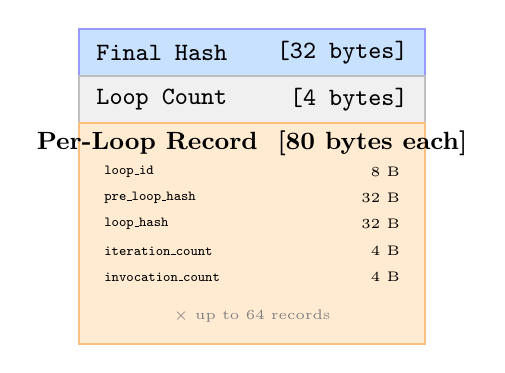
\begin{tikzpicture}[font=\small, node distance=0]
    \draw[fill=hdrblue,draw=blue!40,thick]
      (0,3.6) rectangle (4.4,4.2);
    \node[anchor=west,font=\ttfamily\small] at (0.1,3.9) {Final Hash};
    \node[anchor=east,font=\ttfamily\small] at (4.3,3.9) {[32 bytes]};

    \draw[fill=gray!12,draw=gray!50,thick]
      (0,3.0) rectangle (4.4,3.6);
    \node[anchor=west,font=\ttfamily\small] at (0.1,3.3) {Loop Count};
    \node[anchor=east,font=\ttfamily\small] at (4.3,3.3) {[4 bytes]};

    \draw[fill=loopbg,draw=orange!50,thick]
      (0,0.2) rectangle (4.4,3.0);
    \node[font=\small\bfseries] at (2.2,2.75)
      {Per-Loop Record\ \ [80 bytes each]};
    \node[anchor=west,font=\tiny] at (0.2,2.38) {\texttt{loop\_id}};
    \node[anchor=east,font=\tiny] at (4.2,2.38) {8 B};
    \node[anchor=west,font=\tiny] at (0.2,2.05) {\texttt{pre\_loop\_hash}};
    \node[anchor=east,font=\tiny] at (4.2,2.05) {32 B};
    \node[anchor=west,font=\tiny] at (0.2,1.72) {\texttt{loop\_hash}};
    \node[anchor=east,font=\tiny] at (4.2,1.72) {32 B};
    \node[anchor=west,font=\tiny] at (0.2,1.38) {\texttt{iteration\_count}};
    \node[anchor=east,font=\tiny] at (4.2,1.38) {4 B};
    \node[anchor=west,font=\tiny] at (0.2,1.05) {\texttt{invocation\_count}};
    \node[anchor=east,font=\tiny] at (4.2,1.05) {4 B};
    \node[font=\tiny,gray] at (2.2,0.55) {$\times$ up to 64 records};
  \end{tikzpicture}

  \smallskip
  \centering\small
  Max total: $36 + 64 \times 80 = 5{,}156$~bytes \\[0.3em]
  Syringe pump (4 commands): $1{,}100$~bytes, 14 loops tracked
\end{column}

\end{columns}
\end{frame}

% ══════════════════════════════════════════════════════════════════════════════
% SLIDE 7 — IMPLEMENTATION CHALLENGES
% ══════════════════════════════════════════════════════════════════════════════
\begin{frame}{Implementation Challenges \& Solutions}
\begin{columns}[T]

\begin{column}{0.51\textwidth}
  \textbf{1.\ TEE Parameter Width (32-bit API limit)}\\[0.25em]
  GlobalPlatform TEE value params are 32-bit; BB IDs are 64-bit pointers.\\
  \textit{Fix:} Split each ID across two fields: \texttt{(value.a, value.b)} = \texttt{(lo, hi)}.

  \bigskip
  \textbf{2.\ Debug Buffer Overflow}\\[0.25em]
  Per-node logging to the 16\,KB TEE debug buffer overflowed for complex
  programs — hundreds of ``Debug log overflow'' errors emitted.\\
  \textit{Fix:} Removed per-node logging; rely solely on the final attestation report.

  \bigskip
  \textbf{3.\ Loop Model Mismatch (world-switch count)}\\[0.25em]
  Initial design used explicit \texttt{loop\_enter / loop\_exit / loop\_iteration}
  events per back-edge, adding world switches not present in the BLAST paper count.

  \smallskip
  \begin{tabular}{@{}lrr@{}}
    \toprule
     & \textbf{nbody WS} & \textbf{Loops in report} \\
    \midrule
    Before fix & 25,215,173 & 9 \\
    After fix  & 17,279,130 & 0 \\
    Expected (BLAST) & 17,279,126 & -- \\
    \bottomrule
  \end{tabular}

  \smallskip
  \textit{Fix:} Loop back-edges handled via \texttt{record\_node} only.

  \bigskip
  \textbf{4.\ Deferred Re-initialisation}\\[0.25em]
  After \texttt{finalize()}, pending \texttt{call\_return} events still reference the
  current TA state; a premature \texttt{CMD\_INIT} corrupts them.\\
  \textit{Fix:} \texttt{needs\_reinit} flag defers \texttt{CMD\_INIT} to the next
  \emph{forward} instrumentation call (\texttt{record\_node} / \texttt{call\_enter}).
\end{column}

\begin{column}{0.46\textwidth}
  \textbf{Challenge 2 — buffer overflow screenshot:}\\[0.3em]
  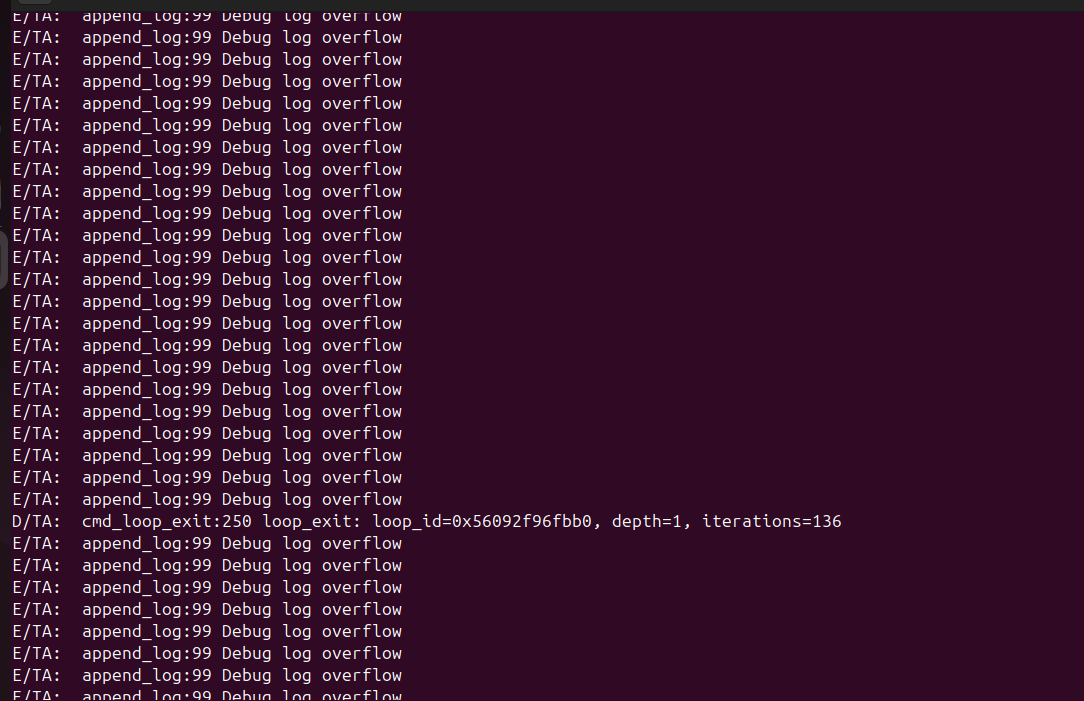
\includegraphics[width=\textwidth]{../screenshots/syringe-pump/buffer_log_overflow.png}

  \bigskip
  \textbf{Challenge 3 — nbody before / after fix:}\\[0.3em]
  \includegraphics[width=\textwidth]%
    {../test-applications/embench-iot-benchmarks/screenshots/cflat_nbody.png}
  \vspace{0.2em}
  {\centering\footnotesize\textit{Before: 25.2M switches, 9 explicit loop records}\\}
  \vspace{0.3em}
  \includegraphics[width=\textwidth]%
    {../test-applications/embench-iot-benchmarks/screenshots/nbody_after_correction.png}
  {\centering\footnotesize\textit{After: 17,279,130 switches — matches Table~2}\\}
\end{column}

\end{columns}
\end{frame}

% ══════════════════════════════════════════════════════════════════════════════
% SLIDE 8 — UNIT TEST RESULTS
% ══════════════════════════════════════════════════════════════════════════════
\begin{frame}{Results: Unit Test Validation on Raspberry Pi~3}

\begin{columns}[T]
\begin{column}{0.48\textwidth}
  \centering
  \textbf{Simple loop — 5 iterations}\\[0.3em]
  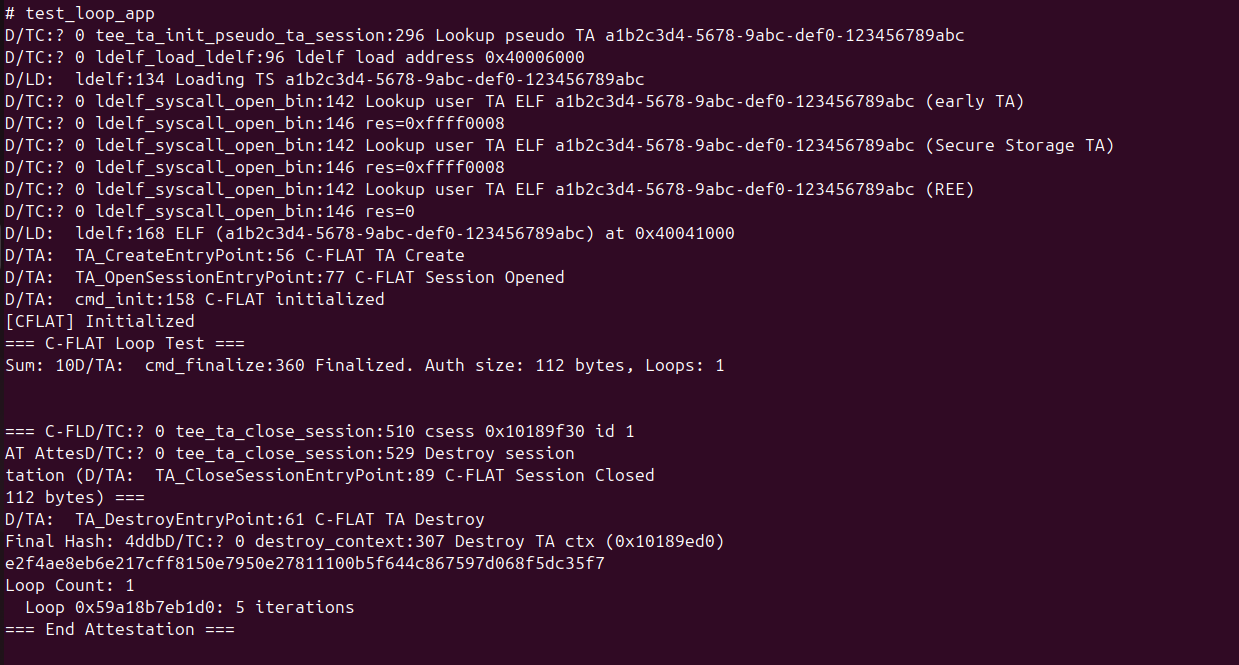
\includegraphics[width=0.88\textwidth]{../screenshots/5_iterations.png}

  \bigskip
  \textbf{Conditional branch — 5 iterations through condition}\\[0.3em]
  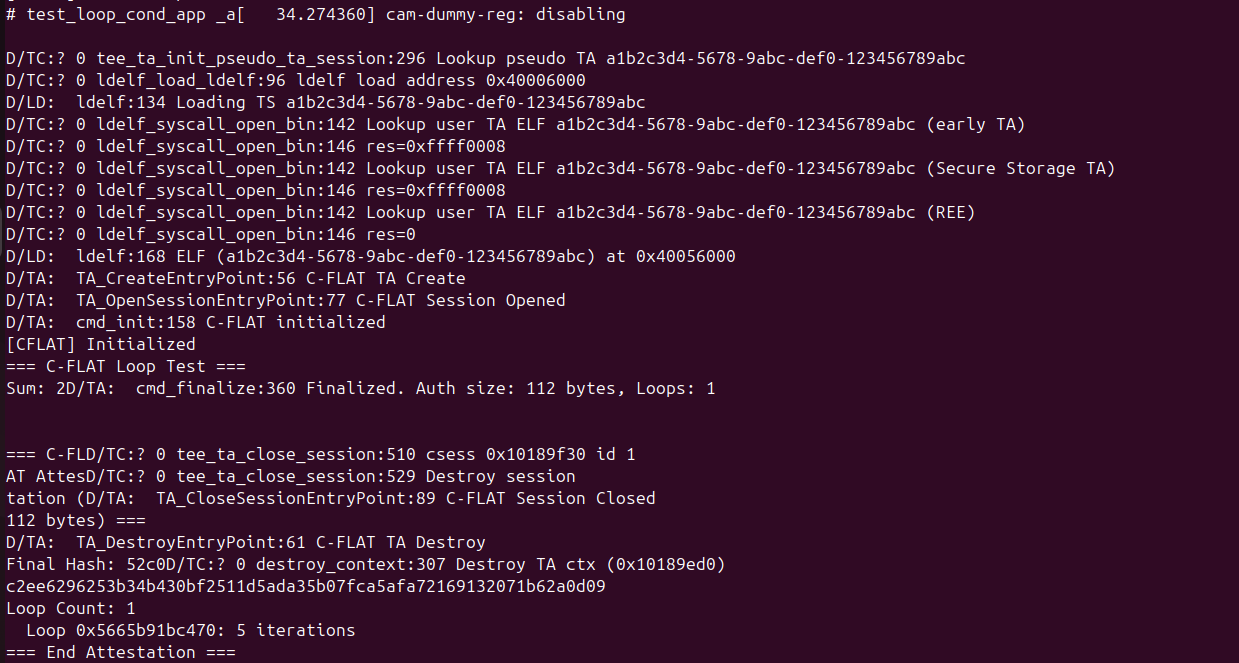
\includegraphics[width=0.88\textwidth]{../screenshots/condition.png}
\end{column}

\begin{column}{0.48\textwidth}
  \centering
  \textbf{Simple loop — 10 iterations}\\[0.3em]
  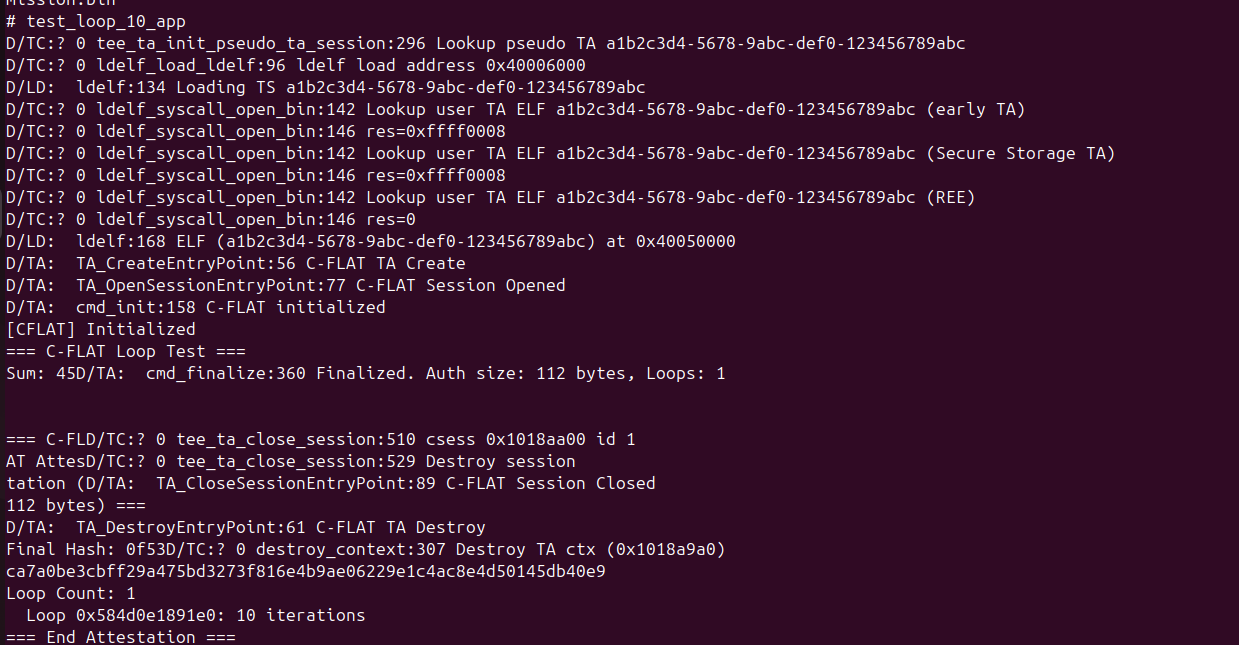
\includegraphics[width=0.88\textwidth]{../screenshots/10_iterations.png}

  \bigskip
  \textbf{Nested loops — outer = 3, inner = 2 per invocation}\\[0.3em]
  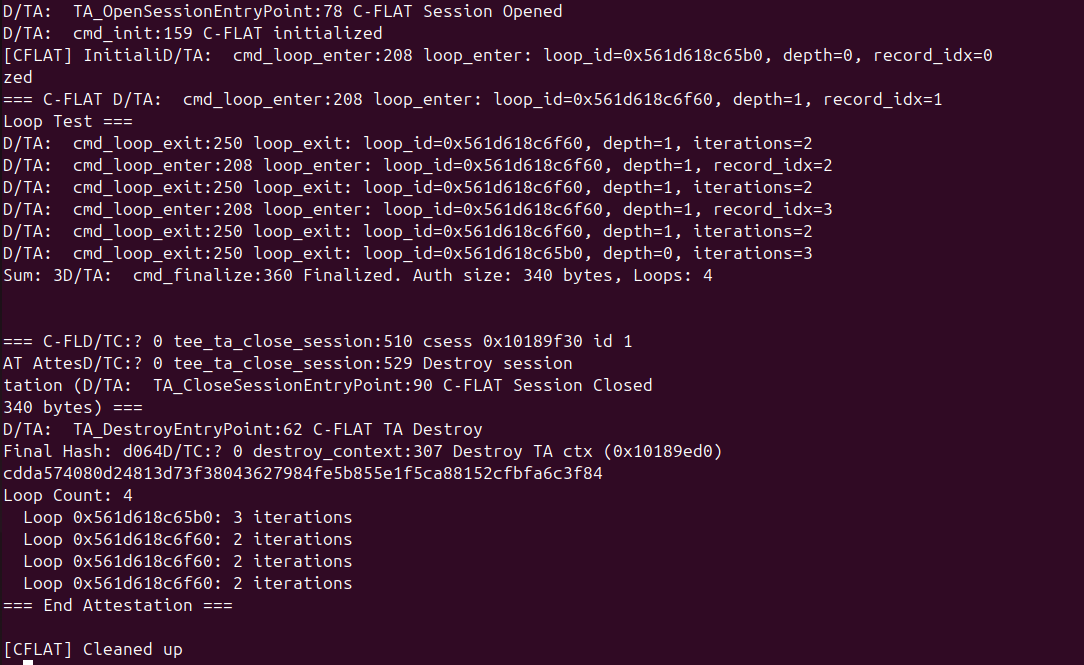
\includegraphics[width=0.88\textwidth]{../screenshots/nested_loops.png}
\end{column}
\end{columns}

\vspace{0.5em}
\begin{block}{}
  \centering\small
  Each test produces a \textbf{unique, deterministic} attestation hash and accurate
  loop records captured in OP-TEE Secure World.
  Changing 5 iterations to 10 produces a completely different final hash.
\end{block}

\end{frame}

% ══════════════════════════════════════════════════════════════════════════════
% SLIDE 9 — SYRINGE PUMP & EMBENCH RESULTS
% ══════════════════════════════════════════════════════════════════════════════
\begin{frame}{Results: Syringe Pump \& Embench-IoT Benchmarks}
\begin{columns}[T]

\begin{column}{0.51\textwidth}
  \textbf{Syringe Pump — cyber-physical integrity}

  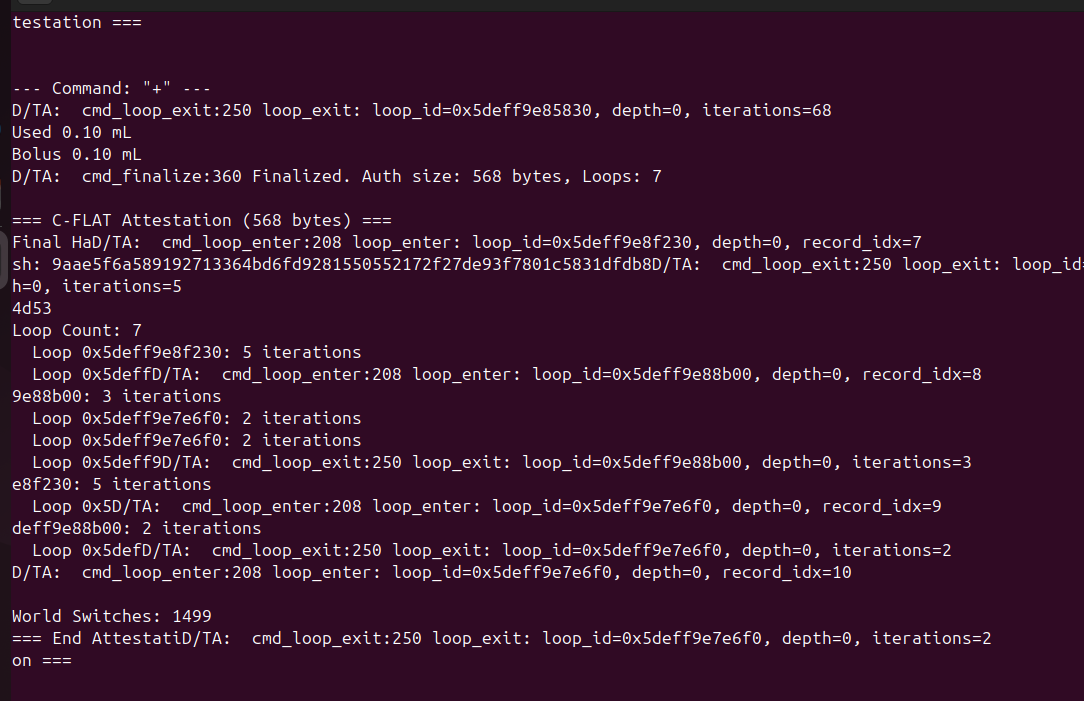
\includegraphics[width=\textwidth]{../screenshots/syringe-pump/command_+.png}

  \smallskip
  \begin{tabular}{@{}lrrr@{}}
    \toprule
    \textbf{Command} & \textbf{Motor Steps} & \textbf{WS} & \textbf{Auth} \\
    \midrule
    \texttt{"10"} (set 10\,µL)  &  0 (set only) & 247  & 340 B \\
    \texttt{"+"}  (push 10\,µL) & \textbf{68}   & 1499 & 568 B \\
    \texttt{"20"} (set 20\,µL)  &  0 (set only) & 1712 & 872 B \\
    \texttt{"+"}  (push 20\,µL) & \textbf{136}  & 4052 & 1100 B \\
    \bottomrule
  \end{tabular}

  \smallskip
  {\small Motor steps $\propto$ fluid volume: linear scaling proven.
  Iteration count in attestation directly proves the physical quantity dispensed.
  Detects data-oriented attacks (loop counter corruption) that CFI cannot.}
\end{column}

\begin{column}{0.46\textwidth}
  \textbf{Embench-IoT: nbody (BLAST Table~2)}

  \includegraphics[width=\textwidth]%
    {../test-applications/embench-iot-benchmarks/screenshots/nbody_after_correction.png}

  \smallskip
  \begin{tabular}{@{}lrr@{}}
    \toprule
    \textbf{Benchmark} & \textbf{Measured WS} & \textbf{Expected (BLAST)} \\
    \midrule
    nbody & 17,279,130 & 17,279,126 \\
    cubic & 2,030,022  & 2,030,022  \\
    \bottomrule
  \end{tabular}

  \smallskip
  \begin{itemize}\small
    \item \textbf{nbody}: $\Delta = +4$ \quad ($< 0.00003\%$)
    \item \textbf{cubic}: exact match
    \item World-switch counts validate the instrumentation
          model against the reference paper implementation
  \end{itemize}

  \bigskip
  \begin{block}{\small Attestation Report (nbody)}
    \footnotesize
    \texttt{Final Hash:}
    \texttt{b4885d944972e7...2eae89}\\
    \texttt{Auth size: 36 bytes, Loops: 0}\\
    \texttt{World Switches: 17,279,130}
  \end{block}
\end{column}

\end{columns}
\end{frame}

% ══════════════════════════════════════════════════════════════════════════════
% SLIDE 10 — CONCLUSION
% ══════════════════════════════════════════════════════════════════════════════
\begin{frame}{Conclusion}
\begin{columns}[T]

\begin{column}{0.54\textwidth}
  \textbf{What was implemented:}
  \begin{itemize}
    \item Full C-FLAT pipeline on RPi3 with OP-TEE: \\
          LLVM Pass $\to$ libcflat $\to$ C-FLAT TA (Secure World)
    \item LLVM IR-level instrumentation of all 4 CFG edge types
          targeting AArch64
    \item SHA-256 hash chain with loop sub-program isolation and
          call-return stack tracking inside OP-TEE
  \end{itemize}

  \medskip
  \textbf{Validated:}
  \begin{itemize}
    \item Unit tests: simple loops, conditional branches, nested loops
    \item Syringe pump: motor step counts prove physical process integrity;
          unique hash per command sequence
    \item Embench-IoT (nbody, cubic): world-switch counts match
          BLAST Table~2 within $< 0.0001\%$
  \end{itemize}

  \medskip
  \textbf{Future Work:}
  \begin{itemize}
    \item Indirect call / virtual dispatch support
    \item Batched TEE invocations to reduce world-switch overhead
    \item Full remote attestation protocol integration
  \end{itemize}
\end{column}

\begin{column}{0.43\textwidth}

  \begin{block}{Key Insight: Iteration Count as Physical Proof}
    \smallskip
    The \textbf{loop iteration count} is the ``smoking gun'' for
    cyber-physical security:
    \begin{itemize}\small
      \item Valid final hash \emph{but} wrong iteration count\\
            $\Rightarrow$ \textbf{data-oriented attack detected}
      \item Bridges the gap between CFI (valid targets only)
            and full execution attestation
    \end{itemize}
  \end{block}

  \medskip
  \begin{exampleblock}{Three Attestation Components}
    \begin{enumerate}\small
      \item \textbf{Final Hash} — correct instruction sequence
      \item \textbf{Loop Iterations} — correct quantity of work done
      \item \textbf{Call Stack} — correct invocation structure
    \end{enumerate}
  \end{exampleblock}

  \medskip
  \begin{alertblock}{Hardware Trust Anchor}
    \small
    All measurements are isolated in ARM TrustZone Secure World
    (OP-TEE). A fully compromised Normal World \emph{cannot}
    modify the attestation report.
  \end{alertblock}

\end{column}

\end{columns}
\end{frame}

\end{document}
